% \paragraph{[2] Inter-dataset $\Delta$.} For inter-dataset $\Delta$ we employ Decision Accuracy (DAcc.; \cite{magnusson2025datadecide}), and Kendall's Tau. DAcc. is an evaluation metric proposed by \cite{magnusson2025datadecide} to quantify the proportion of all possible dataset pairs that are ranked correctly. We use DataDecide \citep{magnusson2025datadecide}, an open-source and -weight benchmark that studies inter-dataset ranking at a small scale of a $n\rightarrow$1.2B. We rank 25 different pre-training datasets using proxy models ranging in size $n \in [3.7\text{M},97.9\text{M}]$. We are unable to use challenging reasoning benchmarks like MATH500 and MMLU Pro as they exhibit significant noise at target scale of 1.2B. Therefore, we use ARC-C and CQA which shows stable cloze form (CF) accuracy \citep{gu-etal-2025-olmes} when averaging 3 seed pre-training runs \citep{gu-etal-2025-olmes}. All results are averages of the two benchmarks. 

% \paragraph{[2] Baselines.} We include five metrics that have been used by existing literature to select pre-training datasets using smaller proxy models: Correct Probability, Normalized Correct Probability, Total Probability, Margin, and 
% CF Accuracy \citep{xie2023doremi, liu2025regmix, magnusson2025datadecide}.

% Our experiments are divided into the following two categories \textbf{[1, 2]} with $n$ $\rightarrow$ $m$ denoting proxy model size $n$ to target model size $m$ where $n, m \in \mbb{N}^+$. Our main experiment is examining \textbf{[1]} intra-dataset $\Delta$ as for \textbf{[2]} inter-dataset $\Delta$, it is highly costly to pre-train $d \in \mbb{N}^+$ number of pre-training datasets at target model size of e.g., 13B, 32B. \textbf{[1]} remains computationally managable as only one target model has to be pre-trained. For \textbf{[2]}, we conduct experiments on a smaller target scale of 1.2B to demonstrate \tsc{rBridge}'s effectiveness in pre-training dataset ranking. 

% \begin{wrapfigure}{r}{0.45\textwidth} 
%   \vspace{-10pt}
%   \centering
%   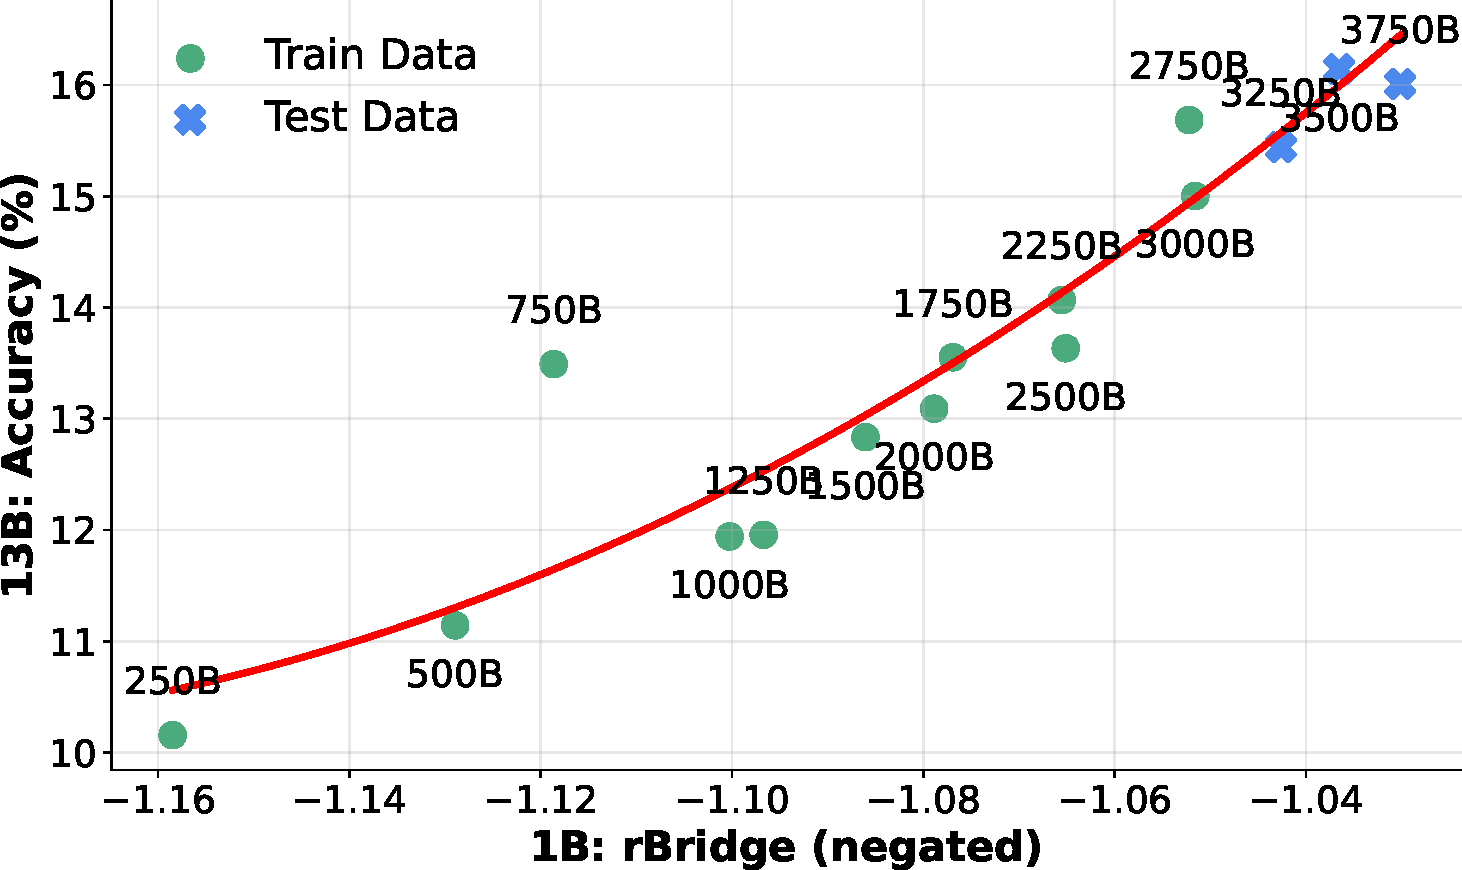
\includegraphics[width=0.45\textwidth]{figs/intra_example.pdf} 
%   \caption{Example visualization of the Intra-dataset $\Delta$ empirical study. This example is on one of the folds evaluating MMLU Pro (STEM).}\label{fig:intra_example} 
%   \vspace{-5pt}
% \end{wrapfigure}

% We examine how well a change in the target scale's Acc. or Pass@K induced by a change in training data size can be predicted by a change of metric value at proxy scale. We set-up the experiments so that the x-axis is a metric at proxy scale, and the y-axis is the target scale's Acc. or Pass@K. Each data point in this relationship corresponds to a certain amount of training data. The data source must be equivalent. See Fig. \ref{fig:intra_example} for an intuitive visualization. To evaluate the effectiveness of the relationship, we employ $5$-fold cross validation following \cite{che2018recurrent}, \cite{lee2020biobert}. Across 5-folds, we report the average curve fitting relationship R$^2$ on the train set and test Mean Absolute Error (MAE; \cite{chai2014root}). 

% We study 1B $\rightarrow$ 13B, and 1B $\rightarrow$ 32B with pre-trained tokens ranging 250 - 3750B tokens with evaluations in intervals of 250B tokens. The pre-training dataset is OLMo-Mix-1124 \citep{olmo20242}. We select six representative reasoning benchmarks spanning mathematics, science, engineering, commonsense, and coding: GSM8K, MATH500, ARC-C \citep{clark2018think}, MMLU Pro \citep{wang2024mmlupro} (STEM subset), CQA \citep{talmor-etal-2019-commonsenseqa}, and HumanEval \citep{chen2021evaluating}.

% We compare six alternatives: Accuracy/Pass@1 (target metric baseline; \citealp{NEURIPS2019_7298332f}), iSFT (intermediate supervised fine-tuning; \citealp{snell2024predicting}), Token Edit Distance (TED; discontinuity-based; \citealp{NEURIPS2023_adc98a26}), Model Probability of Correct Answer (MPCA; continuous, \citealp{NEURIPS2023_adc98a26, snell2024predicting}), and $R^\phi$ (our improved version of ScB; see \textbf{\S\ \ref{sec:align}}).


\section{Empirical Study}\label{sec:exp}

Our experiments are organized in three stages: \textbf{(i)} first, we show that \tsc{rBridge} can be used to rank datasets from proxy scale of $<$100M to target scale 1.2B, \textbf{(ii)} next, we examine the \tsc{rBridge}-target relationship across different amounts of training data at 1B to 32B scale, and \textbf{(iii)} finally, demonstrate that the relationship derived in \textbf{(ii)} can be effectively transferred to a different dataset, allowing us to predict \textit{and} rank large-scale datasets' reasoning performance at a fraction of the cost. 

% Our experiments are organized in three stages: \textbf{(i)} we demonstrate that \tsc{rBridge} effectively ranks datasets using proxy models ($<$100M parameters) to predict performance at target scale (1.2B parameters), \textbf{(ii)} we characterize the \tsc{rBridge}-target relationship across varying training data amounts at 1B--32B scale, and \textbf{(iii)} we show that relationships derived in \textbf{(ii)} transfer zero-shot to different datasets, enabling prediction and ranking of large-scale reasoning performance at substantially reduced computational cost.

\subsection{Experimental Protocol}\label{sec:protocol}

All experimental settings are set \textit{a priori}, and all methods are evaluated in the same manner. Detailed experimental details are available in Appendix \ref{app:setting}.

% \textbf{(i) Dataset Ranking at $<$100M $\rightarrow$ 1.2B.} 
% We follow DataDecide’s \citep{magnusson2025datadecide} protocol to test whether the \tsc{rBridge} score can effectively rank pre-training datasets. Specifically, we rank 25 datasets using proxy models and check whether these rankings align with the target model. Effectiveness is measured by Decision Accuracy (DAcc.; fraction of correctly ordered dataset pairs \citealp{magnusson2025datadecide}) and Kendall’s Tau.

\paragraph{(i) Dataset Ranking at $<$100M $\rightarrow$ 1.2B.} We evaluate whether \tsc{rBridge} scores from proxy models can effectively rank pre-training datasets for target model performance. Following DataDecide's protocol \citep{magnusson2025datadecide}, we rank 25 datasets using proxy models and assess alignment with target model rankings. We measure effectiveness using Decision Accuracy (DAcc.; fraction of correctly ordered dataset pairs; \cite{magnusson2025datadecide}) and Kendall's Tau correlation. Compute cost is measured as FLOPs = $6ND$, where $N$ is model size, and $D$ is dataset size, following \cite{kaplan2020scaling}.

\textbf{Setup.} Proxy models range $n \in [3.7\text{M}, 97.9\text{M}]$, with a 1.2B target model. As discussed in \textbf{\S\ \ref{sec:intro}}, noisy benchmarks such as MATH500 and MMLU Pro are excluded at this scale. Instead, we use ARC-C \citep{clark2018think} and CQA \citep{talmor-etal-2019-commonsenseqa}, which yield stable cloze-form (CF) accuracy \citep{gu-etal-2025-olmes} when averaged across three pre-training seeds \citep{magnusson2025datadecide}. Reported results are the average over these two benchmarks.
\begin{figure}[tb!]
    \centering
    \begin{subfigure}[b]{0.497\textwidth}
        \centering
        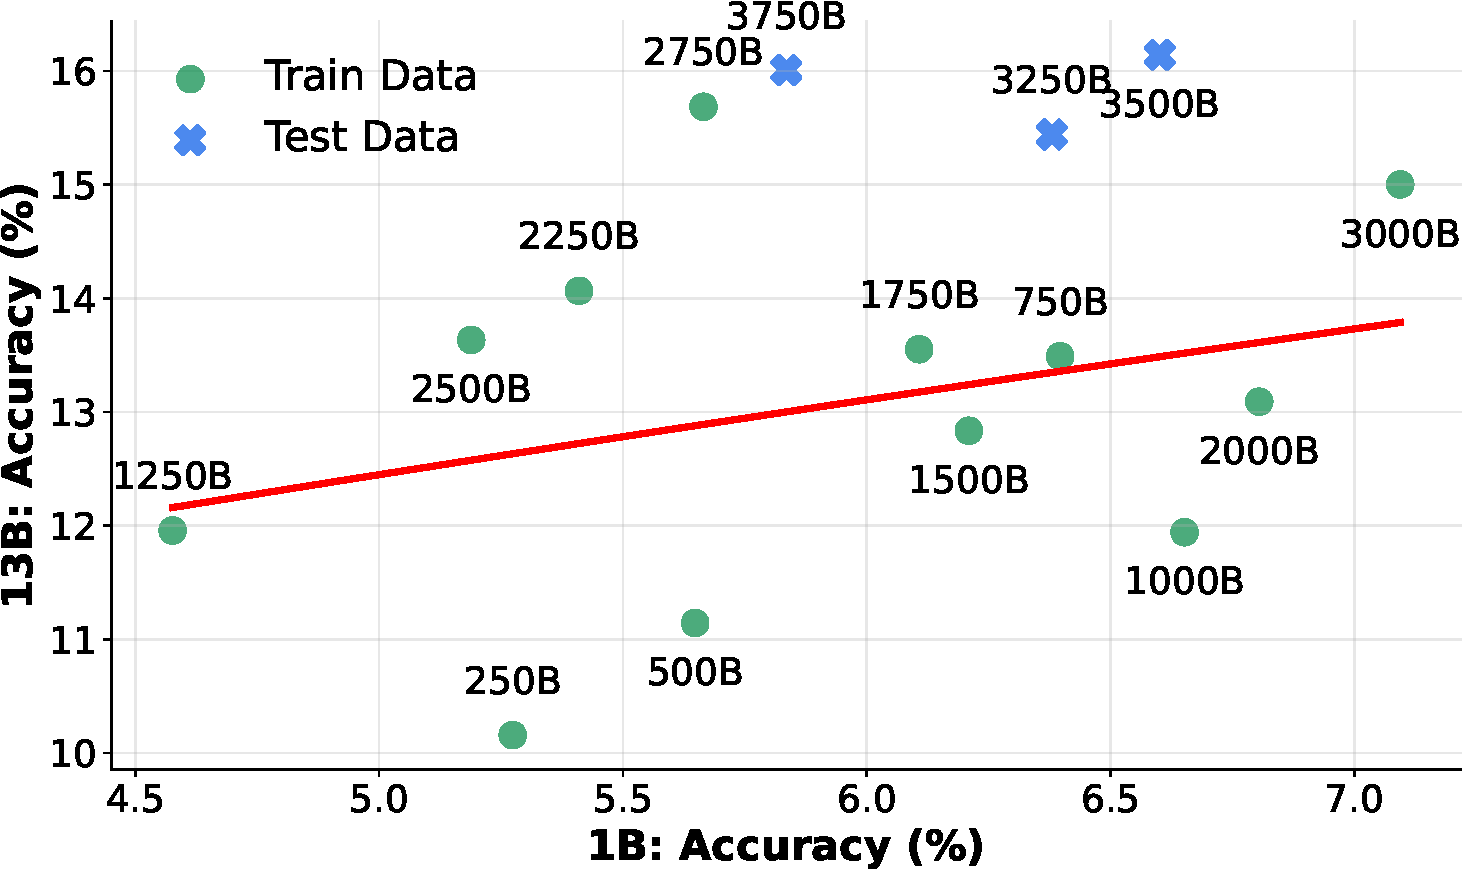
\includegraphics[width=\textwidth]{figs/intra_example_acc.pdf}
        \caption{Target metric Acc. as the proxy metric at 1B.}
        \label{fig:example_acc}
    \end{subfigure}
    \hfill
    \begin{subfigure}[b]{0.497\textwidth}
        \centering
        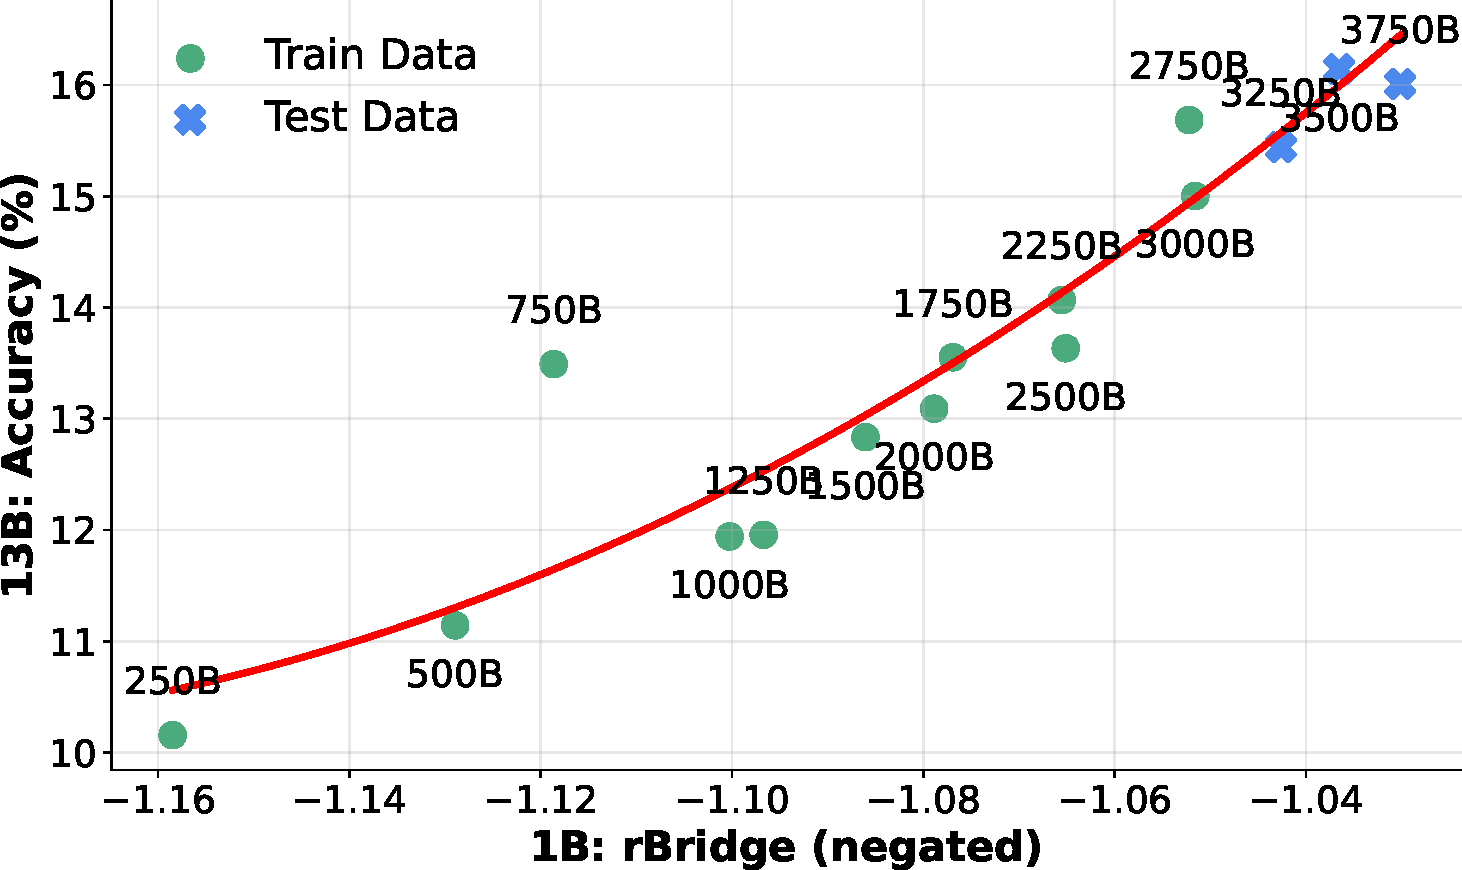
\includegraphics[width=\textwidth]{figs/intra_example.pdf}
        \caption{\tsc{rBridge} as the proxy metric at 1B.}
        \label{fig:example_rbridge}
    \end{subfigure}
    \caption{Example visualization from a fold of proxy-target relationship study at 1B $\rightarrow$ 13B on MMLU Pro (STEM). Each data point represents equal trained tokens for the proxy and target model. Extended visualizations for all other benchmarks available in Appendix \ref{app:more_exp}.}
    \label{fig:intra_example}
\end{figure}

\textbf{Baselines.} Alongside \tsc{rBridge}, we compare five \textit{dataset-ranking} metrics commonly used with proxy models: Correct Probability, Normalized Correct Probability, Total Probability, Margin, and CF Accuracy \citep{xie2023doremi, liu2025regmix, magnusson2025datadecide}.

\paragraph{(ii) Proxy-target Relationship Across Different Amounts of Training Data at 1B $\rightarrow$ 32B.} 

We test whether proxy-scale metrics can predict changes in target-scale Acc. and p@k across different training data sizes. Each data point corresponds to a specific data size from the same source (Fig.~\ref{fig:intra_example}). Following \cite{che2018recurrent}, \cite{lee2020biobert}, we evaluate using 5-fold cross validation on the setup visualized in Fig.~\ref{fig:intra_example}, reporting average train $R^2$ and test Mean Absolute Error (MAE; \cite{chai2014root}). Curve fitting selects the best function based on train $R^2$ from our hypothesis space: linear, quadratic, exponential, and logarithmic. This hypothesis space was defined \textit{a priori} to avoid overfitting. FLOPs 

\textbf{Setup.} We examine model scales of 1B $\rightarrow$ 13B and 1B $\rightarrow$ 32B, pre-trained on 250B to 3750B tokens in 250B token intervals using the OLMo-Mix-1124 dataset \citep{olmo20242}. Evaluation spans six reasoning benchmarks: GSM8K, MATH500, ARC-C, MMLU Pro (STEM subset; \cite{wang2024mmlupro}), CQA, and HumanEval \citep{chen2021evaluating}.

\textbf{Baselines.} We cover six alternative metrics that examine the relationship of small and large models given the \textit{same} data source, and metrics that have shown non-emergent continuity at small scale. First, we include the most naïve approach, the target metric: Accuracy and Pass@1 (Acc./p@1; \cite{NEURIPS2019_7298332f}). Second, we include intermediate supervised fine-tuning (iSFT; \cite{snell2024predicting}) which demonstrates that including a SFT stage throughout the intermediate pre-training checkpoints helps target metric (Acc./p@1) be used as signals. Third is Token Edit Distance (TED; \cite{NEURIPS2023_adc98a26}) which argue that emergence occurs due to discontinuous metrics, and correspondingly proposes their continuous metric. Fourth is Model Probability of Correct Answer (MPCA) as demonstrated in \cite{NEURIPS2023_adc98a26}, \cite{snell2024predicting} as a continuous metric. Last is ScB which visualizes the relationship between ScB and target metric using \textit{numerous} smaller proxy models (similar to the scaling law literature). As mentioned in \textbf{\S\ \ref{sec:rbridge}}, we use our proposed improved version of ScB, R$^\phi$, as there were insufficient details to replicate ScB on all of our benchmarks.

\paragraph{(iii) Zero-shot Functional Relationship Transfer Across Dataset at 1B $\rightarrow$ 7B.} 

Finally, we ask: \textit{if we fit an empirical function on a single pre-training dataset $\mathcal{D}_\text{pre}$ as in} \textbf{(ii)}\textit{, can this function transfer directly to a different dataset $\mathcal{D}_\text{pre}'$}? Concretely, once we fit Acc./p@k $=f(\textsc{rBridge})$ on $\mathcal{D}_\text{pre}$, can this learned function transfer zero-shot (i.e., with no additional fitting) to $\mathcal{D}_\text{pre}'$ where $\mathcal{D}_\text{pre} \neq \mathcal{D}_\text{pre}'$? If so, we could predict the performance (Acc./p@k) of $\mathcal{D}_\text{pre}'$ at target scale using only the proxy model $\pi^\text{p}$, reducing compute by a factor of $m/n$, recalling that $m$, $n$ are the target and proxy sizes, respectively. This allows us to both estimate performance for any number of additional datasets and rank them at a given pre-training size $D_\text{pre}' \in \mbb{N}^+$, simply by inputting the \tsc{rBridge} score in $f(\cdot)$ after training on $D_\text{pre}'$ tokens from $\mathcal{D}_\text{pre}'$.

\begin{figure}[tb!]
    \centering
    \begin{subfigure}[b]{0.497\textwidth}
        \centering
        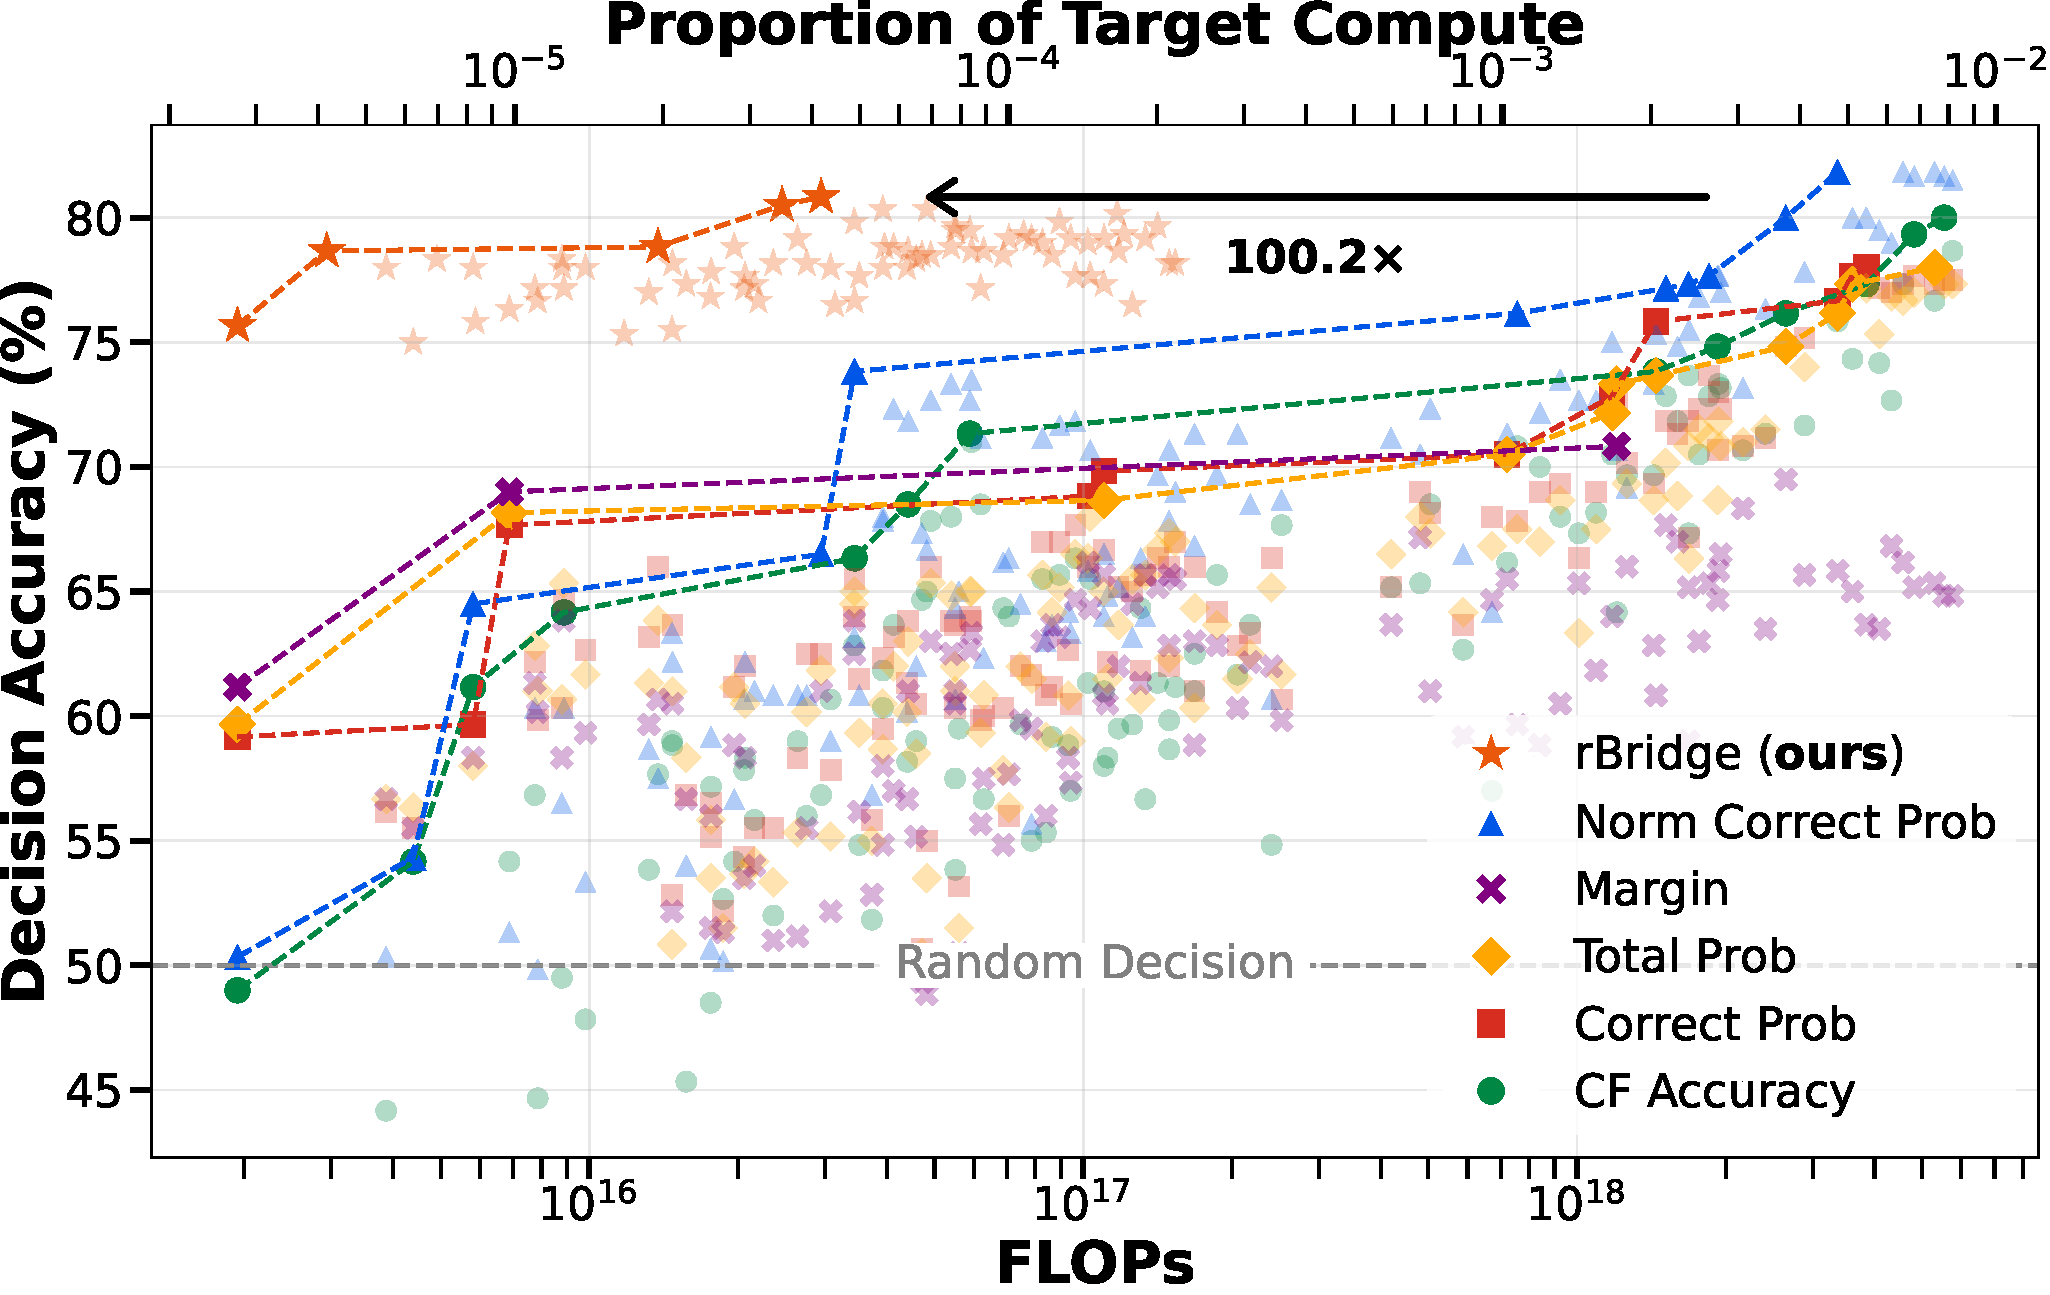
\includegraphics[width=\textwidth]{figs/pareto_decision_accuracy.pdf}
        \caption{Decision Accuracy results across 3.7 - 97.9M proxy model size, and across intermediary checkpoints.}
        \label{fig:pareto}
    \end{subfigure}
    \hfill
    \begin{subfigure}[b]{0.497\textwidth}
        \centering
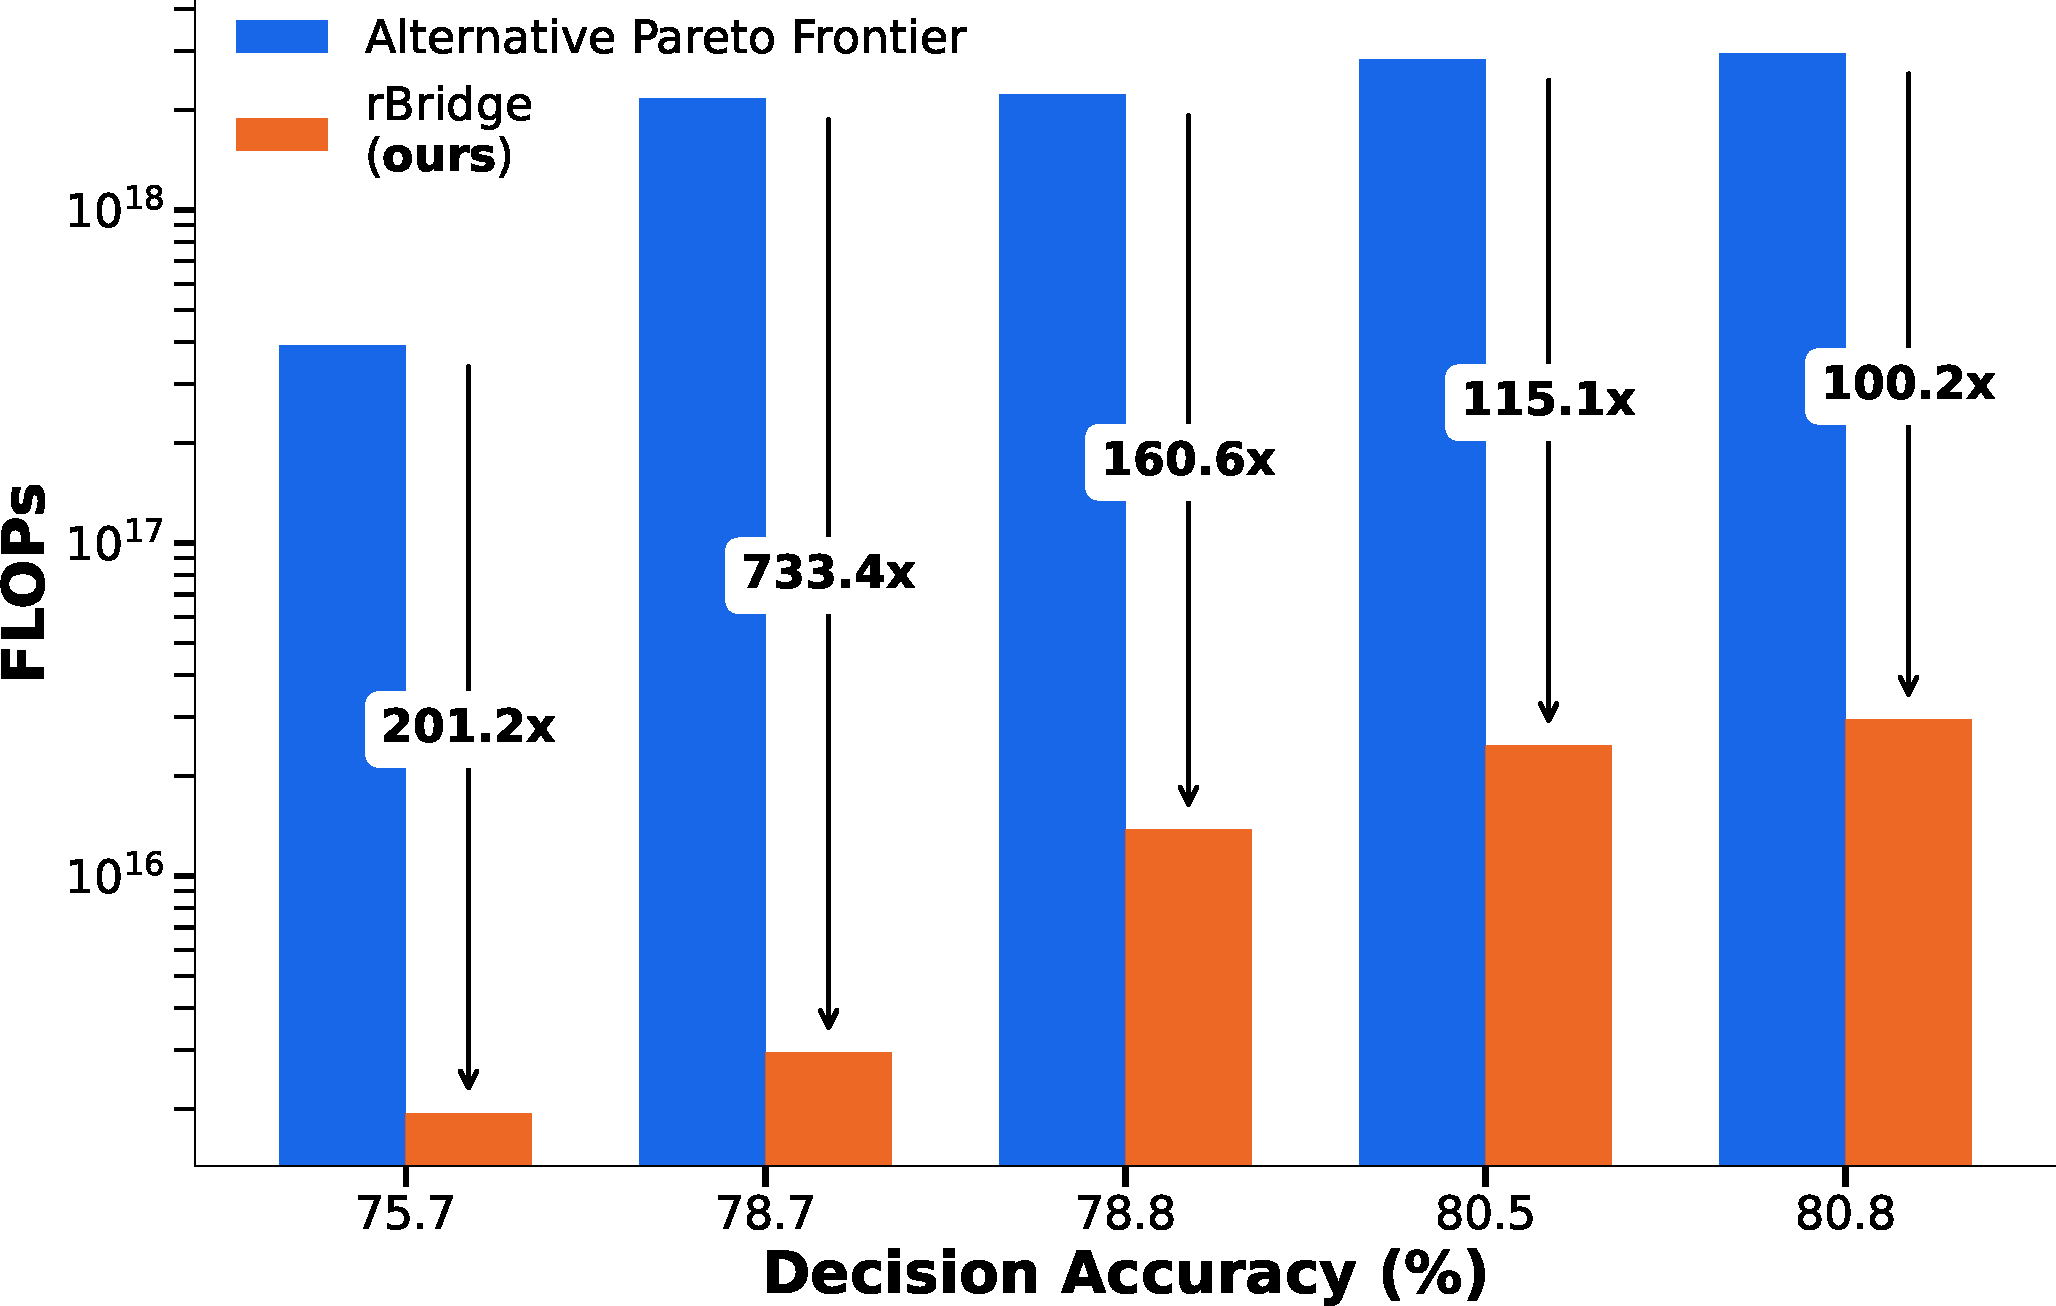
\includegraphics[width=\textwidth]{figs/flops_savings_decision_accuracy.pdf}
        \caption{\tsc{rBridge} saves FLOPs by a factor of 100.2$\times$ to 733.4$\times$.}
        \label{fig:flops}
    \end{subfigure}
    \caption{\tsc{rBridge} improves the pareto frontier in pre-training dataset ranking for 1.2B target model size. Values are averages aggregated across ARC-C and CQA. For intuitive reference, the two most compute efficient points in \tsc{rBridge}'s pareto frontier is (1) 3.7M model size trained on 87.3M tokens, and (2) 6M model size trained on 81.6M tokens.}
    \label{fig:decision_acc}
\end{figure}

\paragraph{Setup.} We curate an additional pre-training dataset $\mc{D}_\text{pre}'$ described in Appendix \ref{app:setting}. Then, we examine how accurate such function as described in \textbf{(ii)}, zero-shot transfers from the OLMo-Mix-1124 to our alternative dataset at 1B $\rightarrow$ 7B at 1T tokens. While larger-scale studies across more model sizes and pre-training datasets would be ideal, training an additional 1B and 7B model for 1T tokens required \textit{thousands} of H100 hours, making further comparisons prohibitively expensive. 

% For instance, at the most compute efficient point representing 3.7M model size trained on 87.3M tokens, \tsc{rBridge} attained DAcc. improvement of +26.7, +25.37, +16.53, +16.03, +14.53, against CF Accuracy, Norm Correct Prob, Correct Prob, Total Prob, and Margin, respectively. This is remarkable as at this proxy compute level, CF Accuracy and Norm Correct Prob displays random decision levels ($\sim$ 50\%). 

% while CF Accuracy and Norm Correct Prob remain near random decision levels ($\sim$50\%). 

% savings FLOPs by a factor of 200.8$\times$ to 920.2$\times$. 

\subsection{Results} \label{sec:result}

\textbf{(i) Over 100$\times$ Dataset Ranking Compute Saving at $<$100M $\rightarrow$ 1.2B.} \tsc{rBridge} significantly improves DAcc. given equivalent compute (Fig. \ref{fig:pareto}). For example, at the most compute-efficient point (3.7M model trained on 87.3M tokens), \tsc{rBridge} achieves up to 27\% higher DAcc. than baseline metrics. This is remarkable as at this proxy compute level, CF Accuracy and Norm Correct Prob displays random decision levels ($\sim$ 50\%). To achieve the same level of DAcc., \tsc{rBridge} uses 100.2$\times$ to 733.4$\times$ less FLOPs (Fig. \ref{fig:flops}).
Kendall’s Tau results are reported in Appendix~\ref{app:more_exp}. As the two evaluation metric are intimately related, the results are highly similar.

\textbf{(ii) Consistently Strongest Relationship at 1B$\rightarrow$13B, 32B.} In 1B $\rightarrow$13B, \tsc{rBridge} achieves the best $R^2$ and MAE in 10/12 cases, and ranks near the top in the remaining two (Tab. \ref{tab:main_tab}). Similar performance occurs in 1B$\rightarrow$13B+SFT where we include a single epoch SFT stage at target scale, and 1B$\rightarrow$32B. For 1B$\rightarrow$13B+SFT and 1B$\rightarrow$32B, granular benchmark-level results appear in Appendix \ref{app:more_exp}.  Aligned with the literature on emergence, discontinuous metrics (Acc./p@1, iSFT) demonstrated worst performance. The remaining continuous metrics performed better, with \tsc{rBridge}'s state-of-the-art performance achieving train $R^2$ of 0.826 - 0.874 and test MAE of 1.304 - 1.481.
\begin{table*}[bt!]
\centering
\resizebox{0.9\textwidth}{!}{%
\begin{tabular}{llcccccc>{\columncolor{gray!15}}c}
\toprule
\textbf{Benchmark} & \textbf{Method:} & \textbf{Acc./p@1} & \textbf{iSFT} & \textbf{TED} & \textbf{MPCA} & \textbf{NLL} & \textbf{R$^\phi$} & \textbf{\tsc{rBridge}} \\
\midrule
\multicolumn{9}{c}{\cellcolor{mybrown!30}\textbf{1B $\rightarrow$ 13B (Pre-to-Pre)}} \\
\midrule
\multirow{2}{*}{GSM8K} & Train R$^2$ & 0.402 & 0.385 & 0.558 & 0.116 & 0.853 & \textbf{0.947} & \underline{0.944} \\
& Test MAE & 5.189 & 4.848 & 5.961 & 84.006 & 3.210 & \underline{1.837} & \textbf{1.751} \\
\midrule
\multirow{2}{*}{MATH500} & Train R$^2$ & 0.127 & 0.076 & 0.213 & 0.025 & 0.861 & \underline{0.864} & \textbf{0.890} \\
& Test MAE & 1.276 & 1.008 & 1.134 & 3.943 & 0.593 & \underline{0.526} & \textbf{0.525} \\
\midrule
\multirow{2}{*}{ARC-C} & Train R$^2$ & 0.200 & 0.166 & 0.547 & 0.319 & 0.166 & \underline{0.950} & \textbf{0.969} \\
& Test MAE & 7.287 & 8.750 & 6.197 & 25.970 & 7.058 & \underline{1.546} & \textbf{1.246} \\
\midrule
\multirow{2}{*}{\makecell{MMLU Pro\\(STEM)}} & Train R$^2$ & 0.167 & --- & 0.199 & 0.200 & \underline{0.207} & \textbf{0.897} & \textbf{0.897} \\
& Test MAE & 1.624 & --- & 1.572 & 1.495 & 12.582 & \underline{0.575} & \textbf{0.574} \\
\midrule
\multirow{2}{*}{CQA} & Train R$^2$ & 0.666 & 0.534 & \underline{0.677} & 0.323 & 0.139 & \textbf{0.890} & \textbf{0.890} \\
& Test MAE & 3.989 & 5.885 & 3.010 & 1697.096 & 5.483 & \underline{2.203} & \textbf{2.182} \\
\midrule
\multirow{2}{*}{HumanEval} & Train R$^2$ & 0.260 & --- & 0.057 & 0.179 & \textbf{0.685} & \underline{0.655} & 0.652 \\
& Test MAE & 2.889 & --- & 2.389 & 3.341 & 2.111 & \underline{2.041} & \textbf{2.025} \\
\midrule
\multicolumn{2}{l}{\textbf{Average Train R$^2$ ($\uparrow$)}} & 0.304 & 0.290 & 0.375 & 0.194 & 0.485 & \underline{0.867} & \textbf{0.874} \\
\multicolumn{2}{l}{\textbf{Average Test MAE ($\downarrow$)}} & 3.709 & 5.123 & 3.377 & 302.642 & 5.173 & \underline{1.455} & \textbf{1.384} \\
\midrule
\multicolumn{9}{c}{\cellcolor{mybrown!30}\textbf{1B $\rightarrow$ 13B + SFT (Pre-to-Post)}} \\
\midrule
\multicolumn{2}{l}{\textbf{Average Train R$^2$ ($\uparrow$)}} & 0.329 & 0.302 & 0.517 & 0.257 & 0.413 & \underline{0.820} & \textbf{0.846} \\
\multicolumn{2}{l}{\textbf{Average Test MAE ($\downarrow$)}} & 4.375 & 5.251 & 4.236 & 27.062 & 3.932 & \underline{1.549} & \textbf{1.304} \\
\midrule
\multicolumn{9}{c}{\cellcolor{mybrown!30}\textbf{1B $\rightarrow$ 32B (Pre-to-Pre)}} \\
\midrule
\multicolumn{2}{l}{\textbf{Average Train R$^2$ ($\uparrow$)}} & 0.312 & 0.349 & 0.352 & 0.205 & 0.488 & \underline{0.820} & \textbf{0.826} \\
\multicolumn{2}{l}{\textbf{Average Test MAE ($\downarrow$)}} & 19.785 & 5.165 & 3.546 & 21.833 & 3.276 & \underline{1.540} & \textbf{1.481} \\
\bottomrule
\end{tabular}
}
\caption{1B$\rightarrow$13B and 1B$\rightarrow$32B performance across mathematics, science, engineering, commonsense, and coding benchmarks. Train fitting and test is done using 5-fold cross validation (\textbf{\S\ \ref{sec:protocol}}). Best value across methods is \textbf{bolded}, and second best is \underline{underlined}.}\label{tab:main_tab}
\end{table*}

% Finally, we ablate the components of \tsc{rBridge} in Fig. \ref{fig:ablation}. Note that we have an ablation study on going from NLL to ScB to R$^\phi$ we propose in \S\ \ref{sec:align}, therefore, skip this part of the ablation study. Here we observe that each part of the \tsc{rBridge} NLL (Eq. \ref{eq:rbridge_nll}) improves performance across all three transfer settings. 

Additionally, even as we increase the proxy model size by 7$\times$, 13$\times$, the target metric fails to out-perform \tsc{rBridge} (Fig. \ref{fig:target_metric}). Notably, \tsc{rBridge}'s and best alternative box-and-whisker's box does not overlap, suggesting a meaningful improvement. To understand where these gains originate, we ablate the components of \tsc{rBridge} in Fig.~\ref{fig:ablation}, showing that each part of the \tsc{rBridge} NLL (Eq.~\ref{eq:rbridge_nll}) plays an important role to its effectiveness across all three experimental settings. Note that we have an ablation study on going from NLL to ScB to R$^\phi$ in \textbf{\S\ \ref{sec:align}}, therefore, skip this part here.

% Similarly, the MinMax normalization stage consistently improves predictive performance as seen by the decrease in MAE, albeit with a lower magnitude of improvement. While the degree of improvement with MinMax normalization may not be large, this provides further evidence that the weighting scheme in Eq. \ref{eq:rbridge_nll} is salient, as the normalization stage amplifies the weight factor's effective where lower weights are given even lower weights, and vice-versa.

\paragraph{(iii) Successful Zero-shot Functional Relationship Transfer at 1B$\rightarrow$7B.} We demonstrate that functions fitted on dataset $\mc{D}_\text{pre}$ with \tsc{rBridge} (from \textbf{(ii)}) can zero-shot transfer to alternative pre-training dataset $\mc{D}_\text{pre}'$, reducing additional experimental compute cost by factor $\frac{m}{n}$ (Tab. \ref{tab:function}). In our experiment setting of 1B$\rightarrow$7B, this yields a 7$\times$ compute reduction since only a proxy model of $\frac{1}{7}$ the target size is required. The transferred function achieves low MAE of 0.043 - 1.417 across most benchmarks (one outlier at 9.716), outperforming $R^\phi$. For dataset ranking using predicted accuracy, \tsc{rBridge} achieves perfect 5/5 performance versus $R^\phi$'s 4/5. This demonstrates that improved function fitting from \textbf{(ii)} translates to superior zero-shot transfer performance across datasets.
\begin{figure}[tb]
    \centering
    \begin{subfigure}[b]{0.497\textwidth}
        \centering
        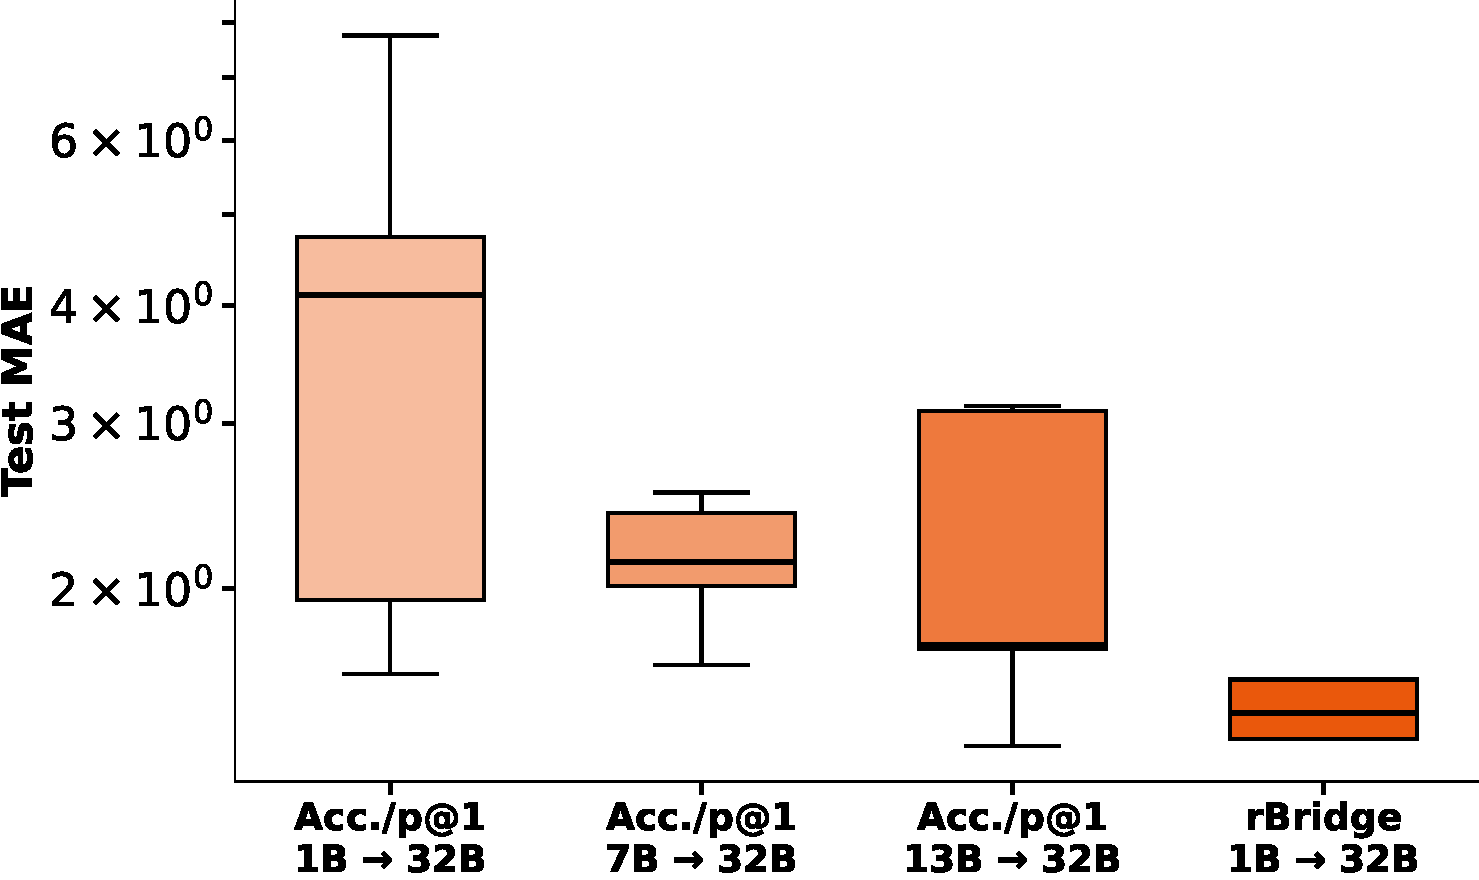
\includegraphics[width=\textwidth]{figs/downstream.pdf}
        \caption{\tsc{rBridge} outperforms proxy models 7 - 13$\times$ larger using the target metric (Acc./p@1).}
        \label{fig:target_metric}
    \end{subfigure}
    \hfill
    \begin{subfigure}[b]{0.497\textwidth}
        \centering
        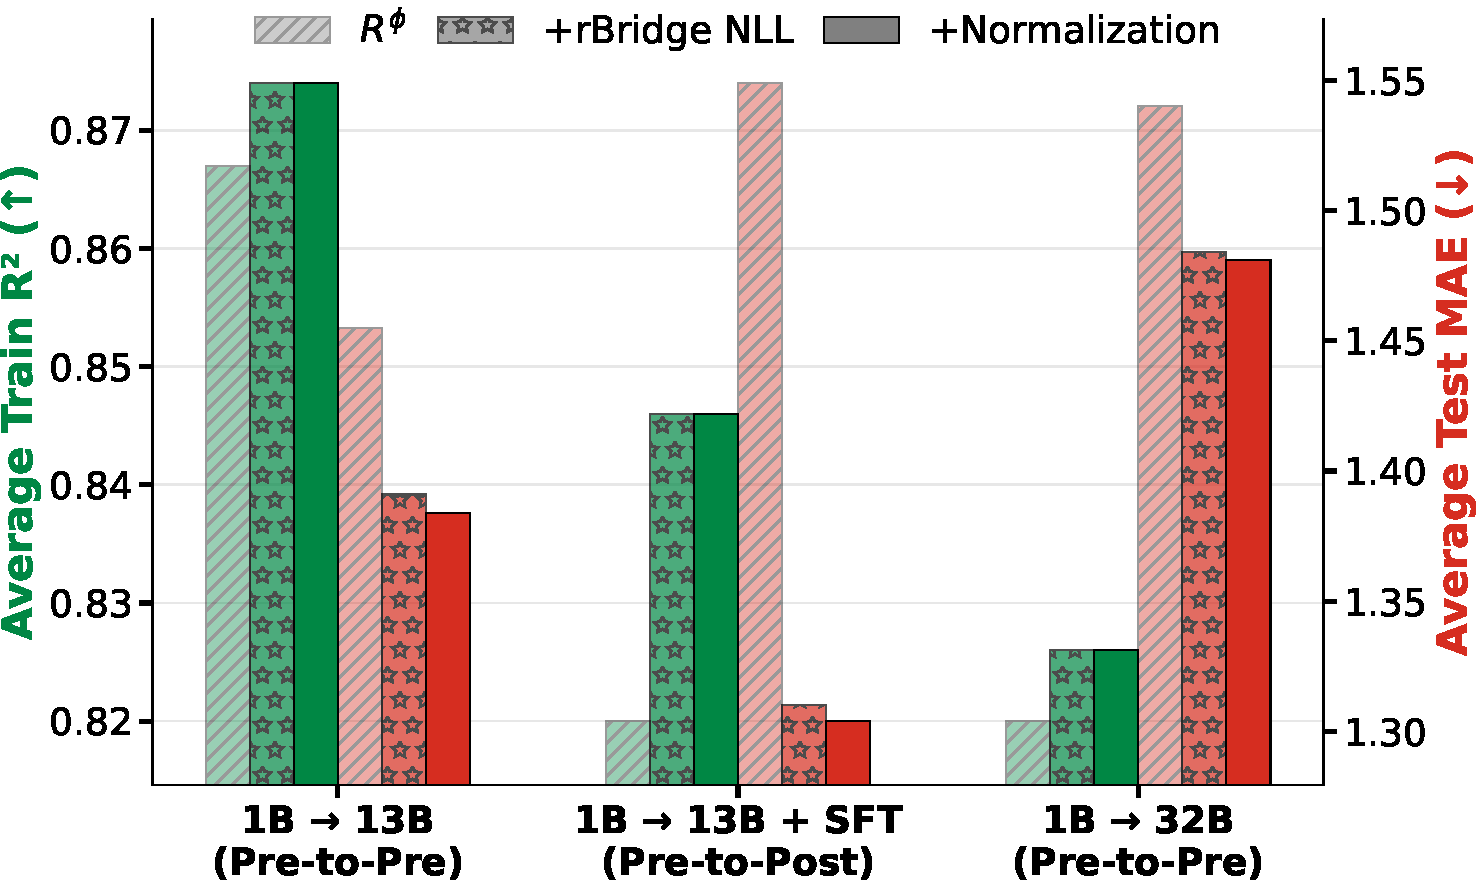
\includegraphics[width=\textwidth]{figs/ablation.pdf}
        \caption{Ablation shows that \tsc{rBridge} NLL and normalization results in consistent improvement.}
        \label{fig:ablation}
    \end{subfigure}
    \caption{Additional experimental results demonstrate clear advantages of our proposed method.}
    \label{fig:additional}
\end{figure}


\begin{table*}[tb]
\centering
\resizebox{\textwidth}{!}{
\begin{tabular}{l|l|ccccc|c}
\toprule
\multicolumn{8}{c}{\cellcolor{mybrown!30}\textbf{1B $\rightarrow$ 7B Zero-shot Functional Relationship Transfer from $\mc{D}_\text{pre}$ to $\mc{D}'_\text{pre}$}} \\
\midrule
\textbf{Method} & \textbf{Benchmark:} & \textbf{GSM8K} & \textbf{MATH500} & \textbf{ARC-C} & \textbf{MMLU Pro} & \textbf{CQA} & \textbf{Average} \\
\midrule
\multirow{2}{*}{\textbf{Ground Truth}} & \textbf{Acc. (\%) of $\mc{D}_\text{pre}$} & \cellcolor{mygreen!30}10.538 & \cellcolor{myred!30}2.800 & \cellcolor{mygreen!30}56.911 & \cellcolor{mygreen!30}10.225 & \cellcolor{mygreen!30}60.442 & 28.183\\
 & \textbf{Acc. (\%) of $\mc{D}_\text{pre}'$} & \cellcolor{myred!30}8.264 & \cellcolor{mygreen!30}3.600 & \cellcolor{myred!30}51.536& \cellcolor{myred!30}9.578 & \cellcolor{myred!30}44.554 & 23.506 \\
 \midrule
\multirow{3}{*}{\textbf{R$^\phi$}} & \textbf{Acc. (\%) Prediction of $\mc{D}_\text{pre}'$} & 9.886 & 3.116 & 52.558 & 10.649 & 57.479 & 26.738 \\
 & \cellcolor{gray!30}\textbf{Rank($\mc{D}_\text{pre}$, $\mc{D}_\text{pre}'$) w. Prediction ($\uparrow$)} & \cellcolor{gray!30}\textcolor{mygreen}{\checkmark} & \cellcolor{gray!30}\textcolor{mygreen}{\checkmark}& \cellcolor{gray!30}\textcolor{mygreen}{\checkmark} & \cellcolor{gray!30}\textcolor{myred}{\texttimes} & \cellcolor{gray!30}\textcolor{mygreen}{\checkmark} & \cellcolor{gray!30}4/5 \\
 & \cellcolor{gray!30}\textbf{MAE ($\downarrow$)} & \cellcolor{gray!30}1.622 & \cellcolor{gray!30}0.484 & \cellcolor{gray!30}1.022 & \cellcolor{gray!30}1.071 & \cellcolor{gray!30}12.926 & \cellcolor{gray!30}3.425 \\
  \midrule
\multirow{3}{*}{\textbf{rBridge}} & \textbf{Acc. (\%) Prediction of $\mc{D}_\text{pre}'$} & 8.220 & 3.044 & 52.254 & 8.161 & 54.269 & 25.190 \\
 & \cellcolor{gray!30}\textbf{Rank($\mc{D}_\text{pre}$, $\mc{D}_\text{pre}'$) w. Prediction ($\uparrow$)} & \cellcolor{gray!30} \textcolor{mygreen}{\checkmark} & \cellcolor{gray!30} \textcolor{mygreen}{\checkmark}& \cellcolor{gray!30}\textcolor{mygreen}{\checkmark} & \cellcolor{gray!30}\textcolor{mygreen}{\checkmark} & \cellcolor{gray!30}\textcolor{mygreen}{\checkmark} & \cellcolor{gray!30} \textbf{5/5} \\
 & \cellcolor{gray!30}\textbf{MAE ($\downarrow$)} & \cellcolor{gray!30} 0.043 & \cellcolor{gray!30}0.556 & \cellcolor{gray!30}0.718 & \cellcolor{gray!30}1.417 & \cellcolor{gray!30}9.716 & \cellcolor{gray!30} \textbf{2.490} \\
\bottomrule
\end{tabular}
}
\caption{\tsc{rBridge} demonstrates strong zero-shot functional relationship transfer across datasets. Ground Truth rows are the Acc. performance and ranking ({\setlength{\fboxsep}{2pt}\colorbox{mygreen!30}{rank 1}, \colorbox{myred!30}{rank 2}}) that the prediction is aiming to attain. \tsc{rBridge} achieves 0 - 1.5 (\%) error-rate excluding one outlier, and perfectly ranks the datasets on all five benchmarks. Average values are aggregated across the row. }\label{tab:function}
\end{table*}

% \paragraph{[1] Intra-dataset $\Delta$.} For intra-dataset $\Delta$ we employ $5$-fold cross validation following \cite{che2018recurrent}, \cite{lee2020biobert}. Across 5-folds, we report the average curve fitting relationship R$^2$ on the train set and test Mean Absolute Error (MAE; \cite{chai2014root}). The proxy to target model scale we examine is 1B $\rightarrow$ 13B, 32B, with pre-trained tokens ranging 250 - 3750B tokens with evaluations in intervals of 250B tokens. We also include a Pre-to-Post study which examines how well the proxy model can predict pre-trained models with an additional SFT stage. The pre-training dataset is OLMo-Mix-1124 \citep{olmo20242}. We select six representative reasoning benchmarks spanning mathematics, science, engineering, commonsense, and coding: GSM8K, MATH500, ARC-C \citep{clark2018think}, MMLU Pro \citep{wang2024mmlupro} (STEM subset), CQA \citep{talmor-etal-2019-commonsenseqa}, and HumanEval \citep{chen2021evaluating}.

% \paragraph{[1] Baselines.} We cover 6 alternative metrics that examine the relationship of small and large models given the same data source, and metrics that have shown non-emergent continuity at small scale. First, we include the most naïve approach, the target metric: Accuracy and Pass@1 (Acc./p@1; \cite{NEURIPS2019_7298332f}). Second, we include intermediate supervised fine-tuning (iSFT; \cite{snell2024predicting}) which demonstrate that including a SFT stage throughout the intermediate pre-training checkpoints help target metric (Acc./p@1) be used as signals in smaller models with less training compute. Third is Token Edit Distance (TED; \cite{NEURIPS2023_adc98a26}) which showed that emergence occurs due to discontinuous metrics. Fourth is Model Probability of Correct Answer (MPCA) as demonstrated in \cite{NEURIPS2023_adc98a26}, \cite{snell2024predicting} as a continuous metric. Last is ScB which visualize the relationship between ScB and target metric using multi-scale smaller models. As mentioned in \S\ \ref{sec:target_align}, we use our proposed improved version of ScB, R$^\phi$, as there were insufficient details to replicate ScB on all of our benchmarks.

% A final challenge in using ScB as a baseline is the lack of instructions to replicate their method for benchmarks' $Y^*$ that they have not released. For instance, while we want to evaluate on GSM8K, we do not have a followable format for generating the $Y^*$ as their HuggingFace dataset indicate a \textit{unique} instruction format for each benchmark. 
